\documentclass[12pt,a4paper]{article}
\usepackage{physics}
\usepackage{amssymb, amsmath, graphicx}
\usepackage{subcaption}
\usepackage{svg}
\svgpath{{svg/}}
\newcommand{\activity}{Activity 17 -- Neural Networks}
\input{spp.dat}

\begin{document}

\title{\TitleFont \activity}
\author[ ]{\textbf{Kenneth V. Domingo} \\
2015--03116 \\
App Physics 186, 1\textsuperscript{st} Semester, A.Y. 2019--20}
\affil[ ]{\corremail{kvdomingo@up.edu.ph} }

\maketitle
\thispagestyle{titlestyle}

\section*{Results and Discussion}
\setcounter{section}{1}
\subsection{Function fitter}
For this activity \cite{soriano}, we will first explore the applications of a neural network---or more accurately, a multilayer perceptron (MLP)---as a universal function fitter. Designing an neural network architecture can be quite tedious as there are a lot of hyperparameters to tune in order for you to get desired results. After several attempts of trial-and-error, I ended up with the network shown in Fig. \ref{fig:funcfit-architecture} (all network visualizations were done using \cite{nn-svg}). For the training data, I generated 1000 random numbers distributed uniformly in the range $[-1, 1]$ as the input, and the corresponding function as the output. Specifically, the functions used were:

\begin{itemize}
	\item linear: $f(x) = x$
	\item quadratic: $f(x) = x^2$
	\item cubic: $f(x) = x^3$
	\item $\tanh(x)$
	\item logistic sigmoid: $\frac{1}{1 + \exp[-x]}$
	\item $\sin(2\pi fx)$
\end{itemize}

\begin{figure}[htb]
	\centering
	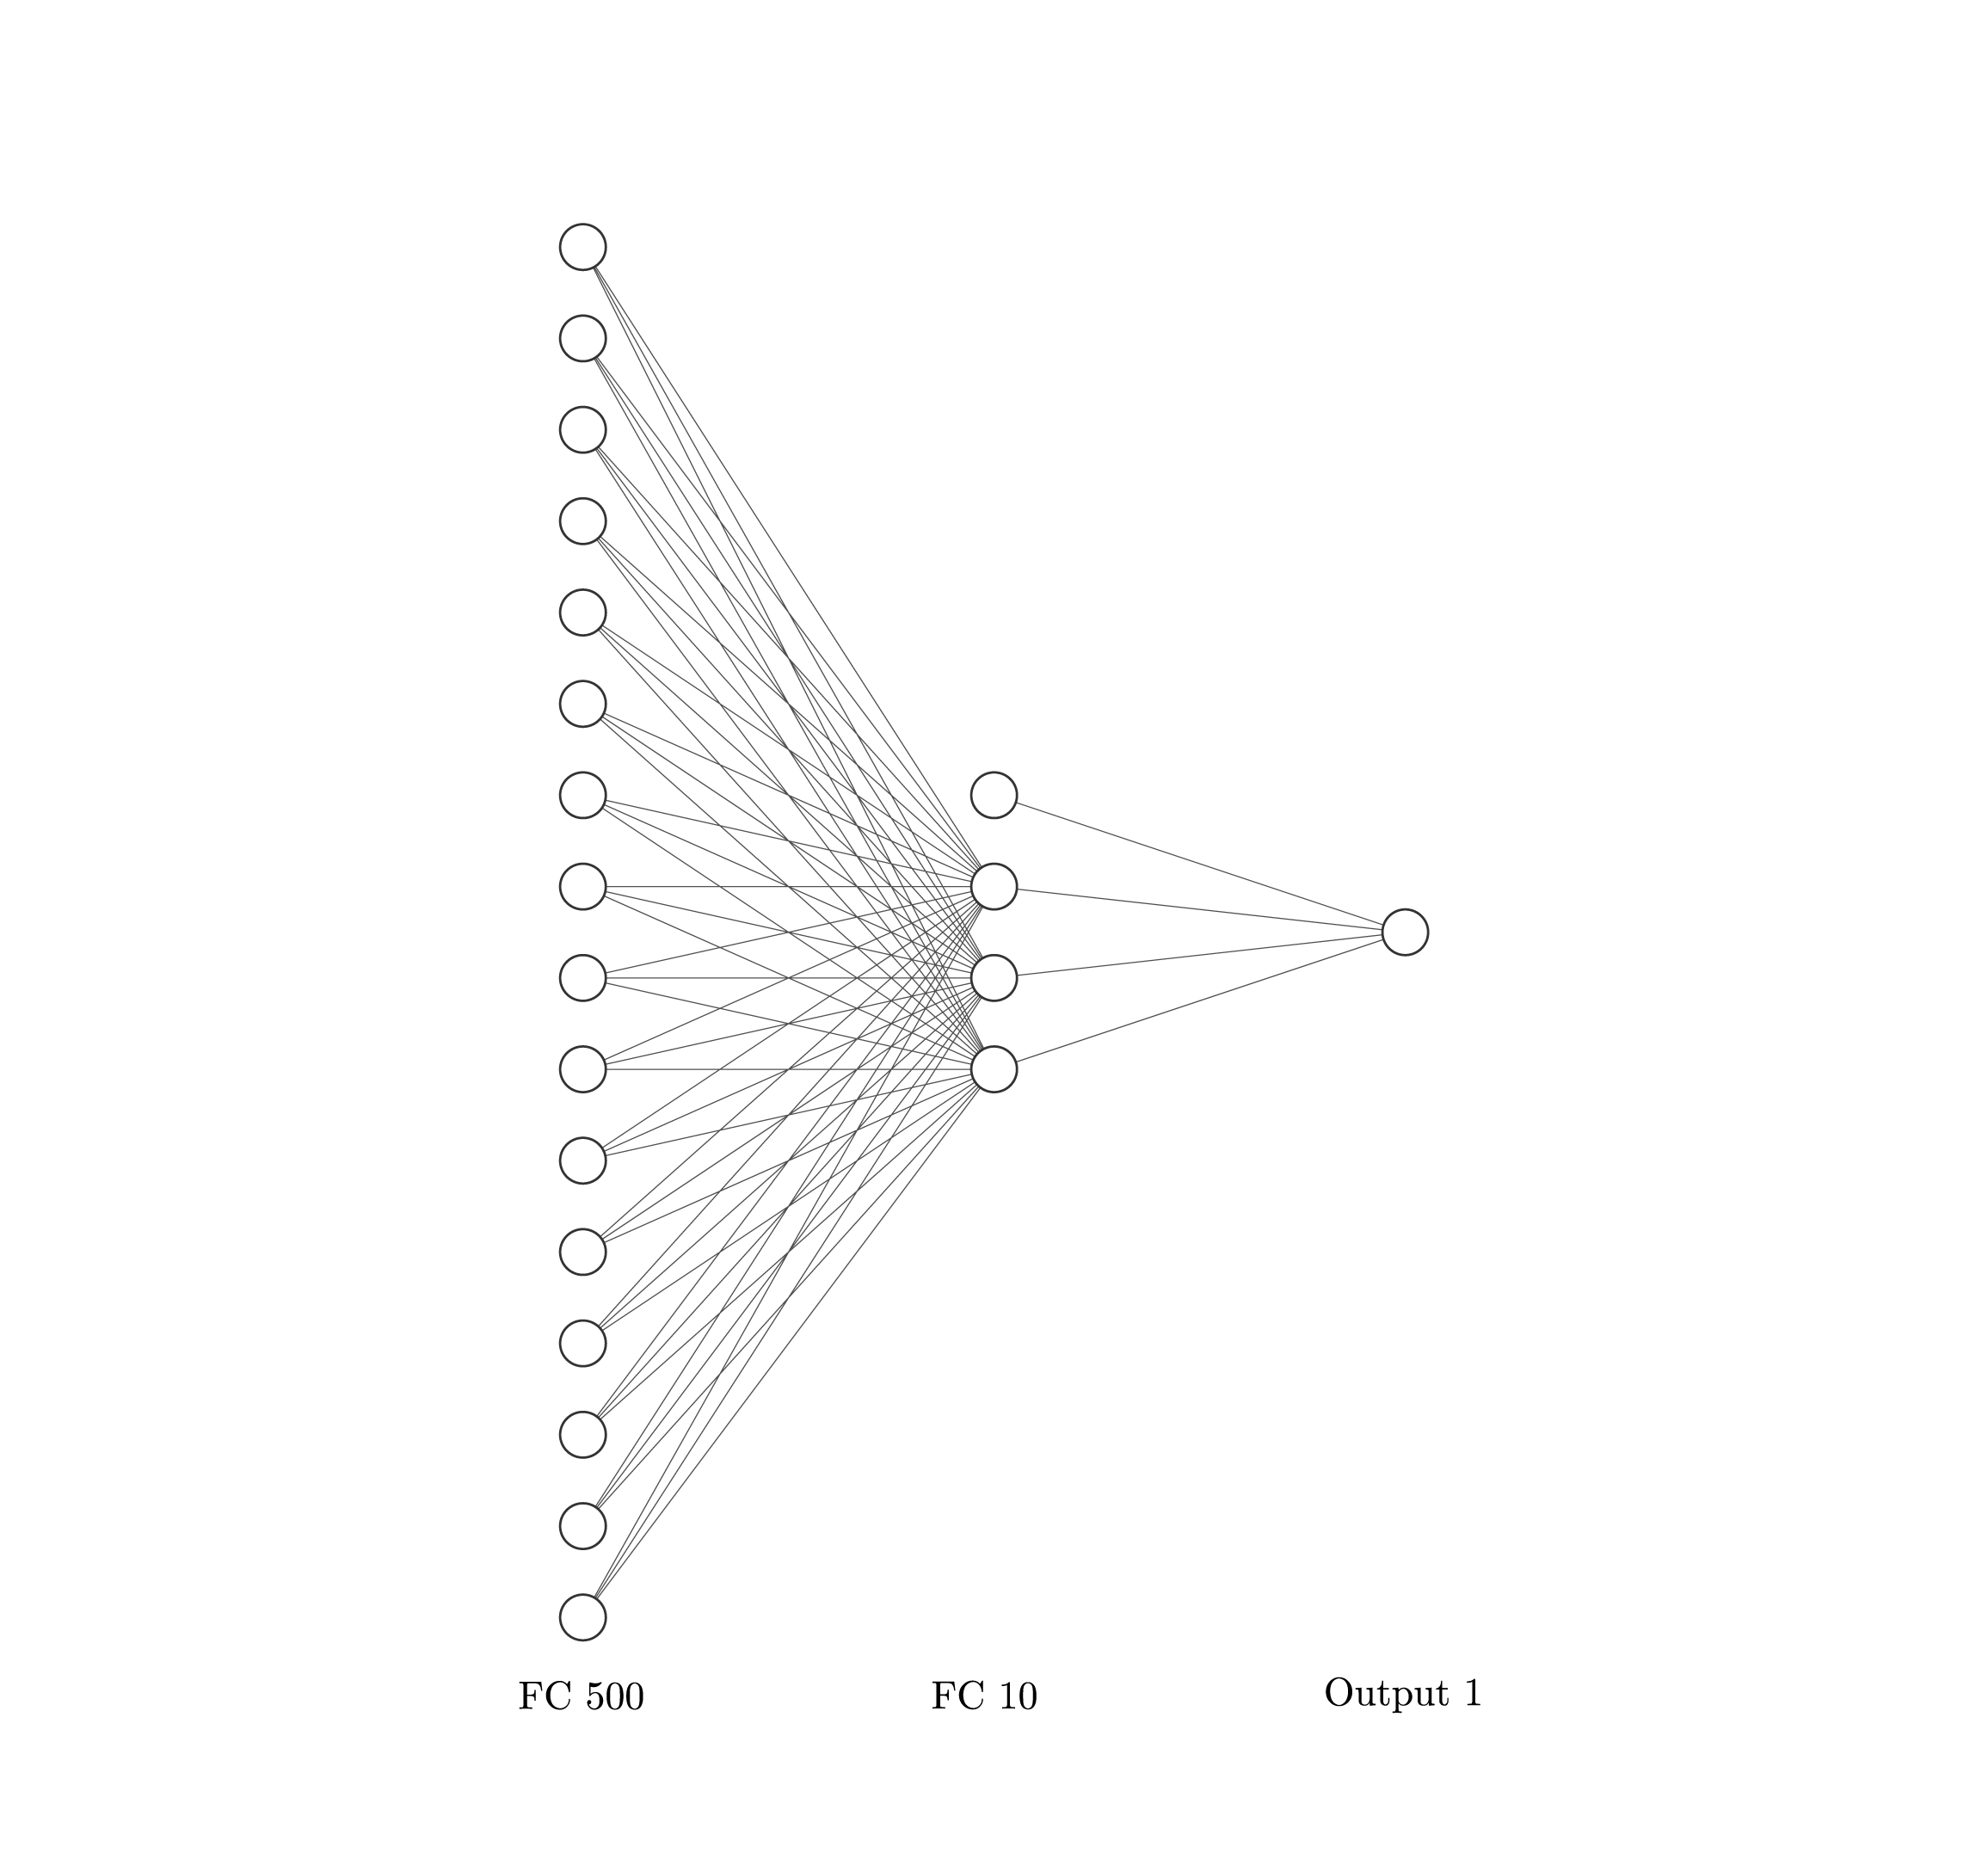
\includegraphics[width=0.75\textwidth]{func-fit.png}
	\caption{Network architecture for the function fitter.}
	\label{fig:funcfit-architecture}
\end{figure}

\begin{figure}[htb]
	\centering
	\begin{subfigure}[h!]{0.3\textwidth}
		\centering
		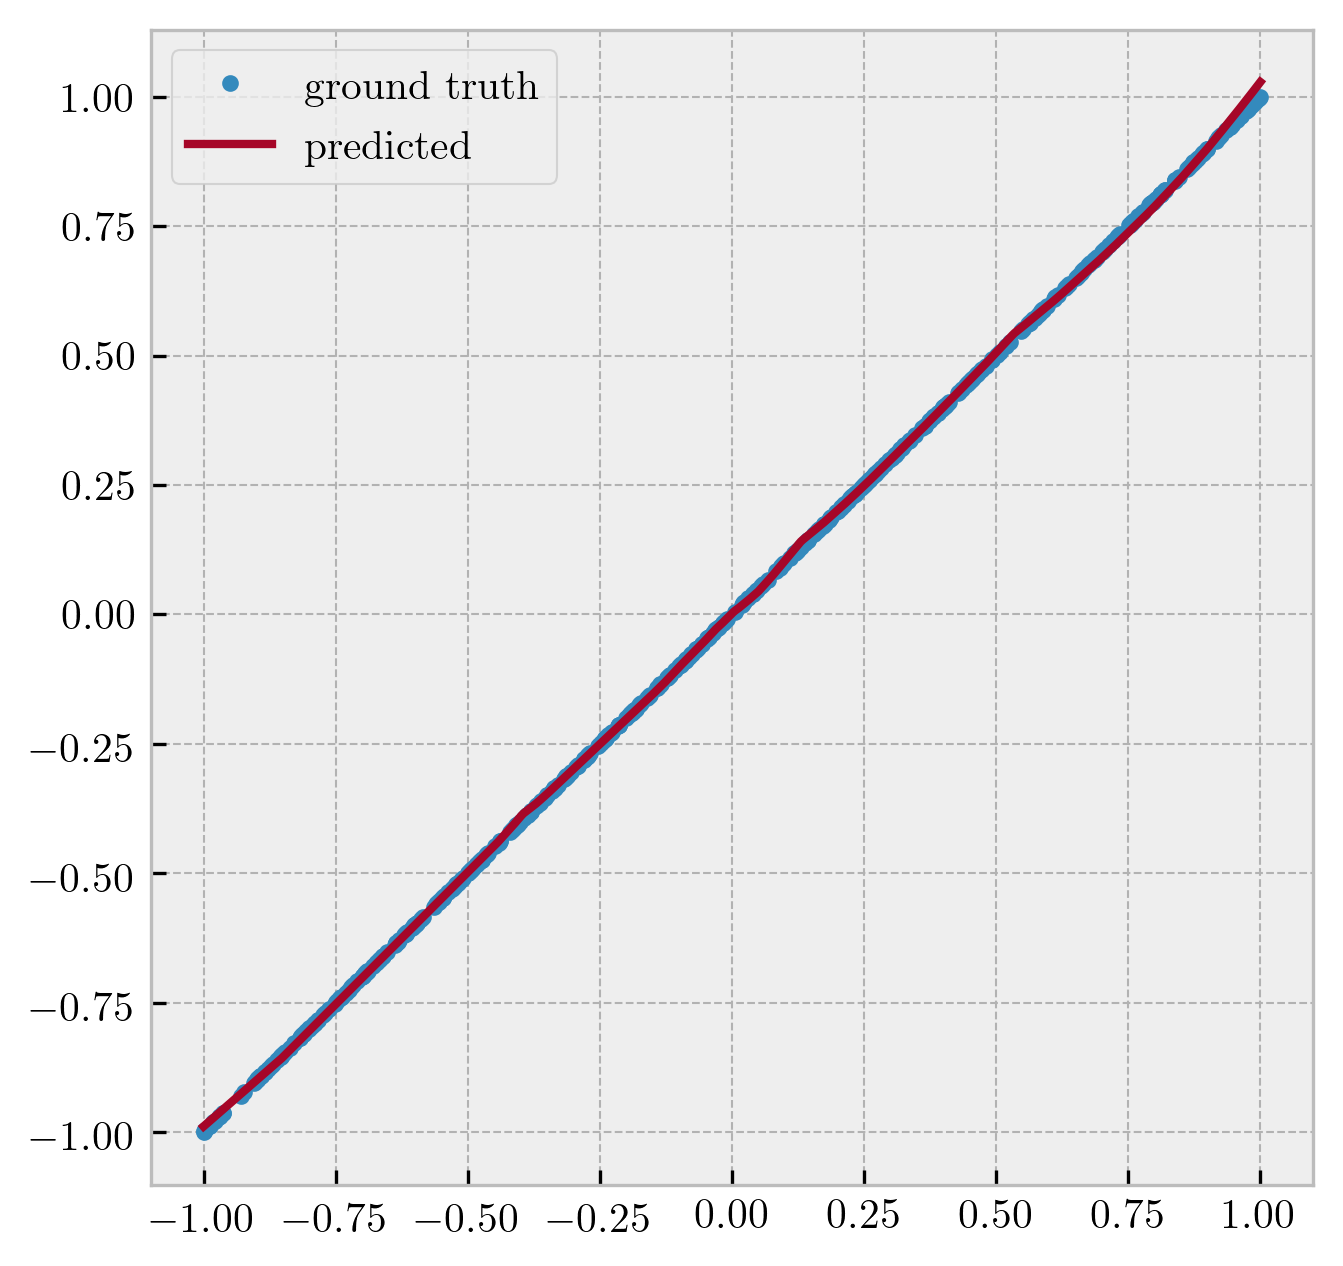
\includegraphics[width=\textwidth]{fit-1-pred.png}
		\caption{linear}
		\label{fig:linear}
	\end{subfigure}
	\begin{subfigure}[h!]{0.3\textwidth}
		\centering
		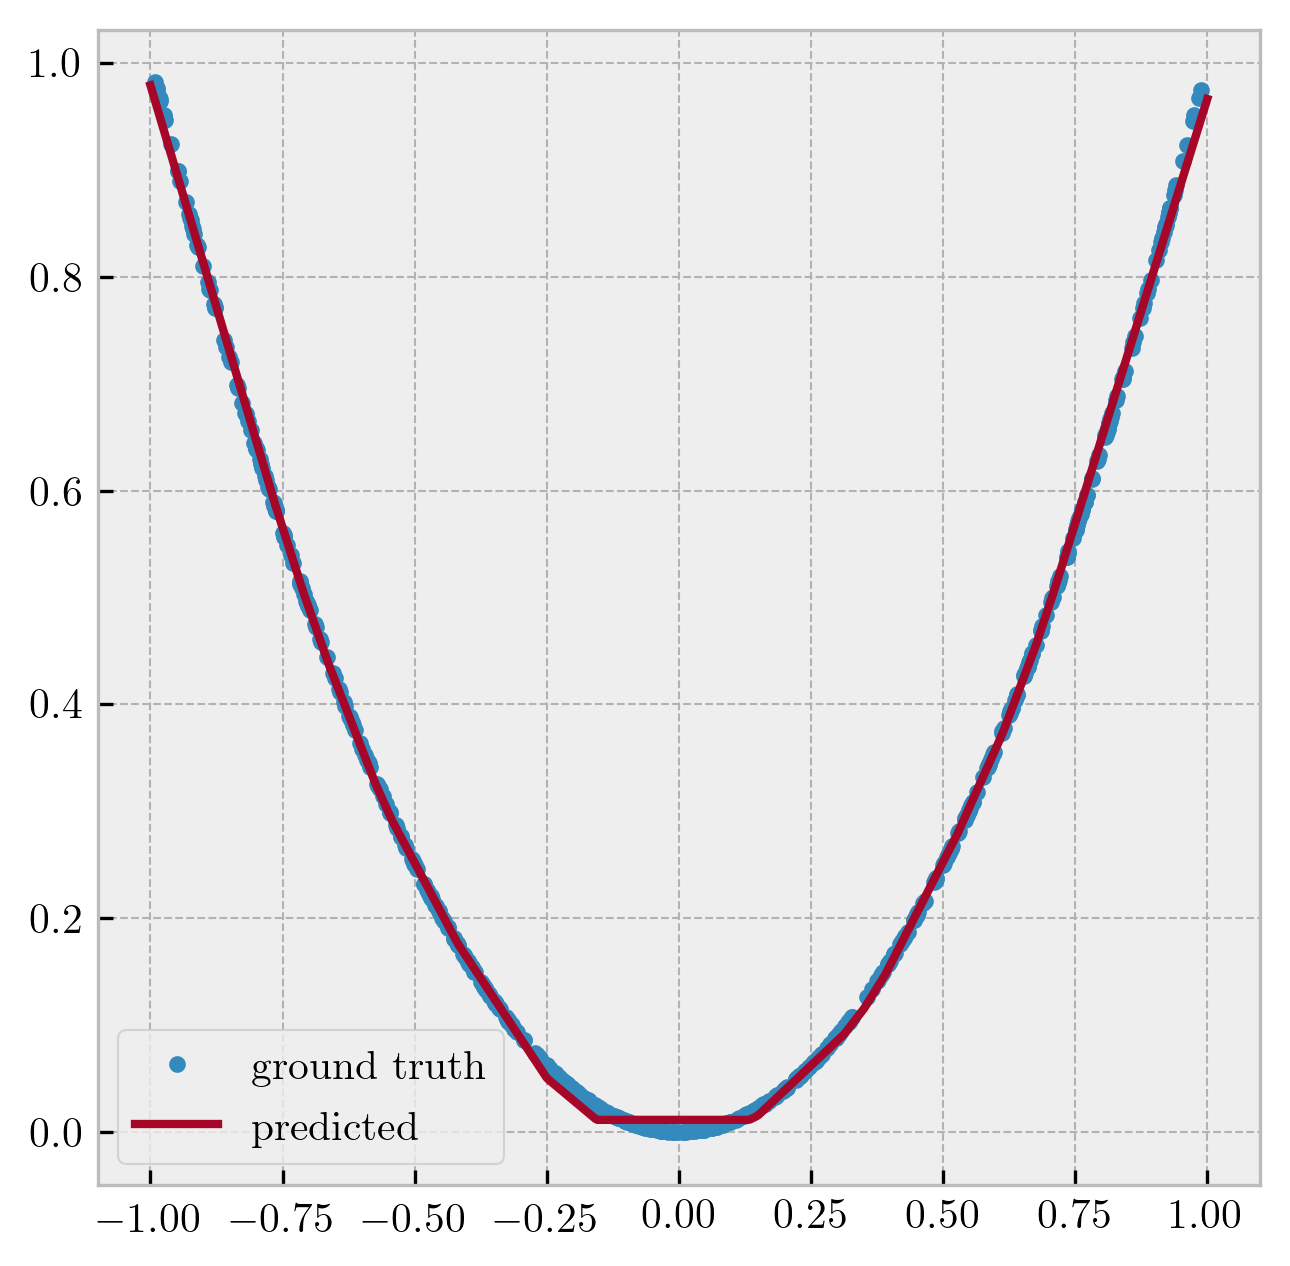
\includegraphics[width=\textwidth]{fit-2-pred.png}
		\caption{quadratic}
		\label{fig:quadratic}
	\end{subfigure}
	\begin{subfigure}[h!]{0.3\textwidth}
		\centering
		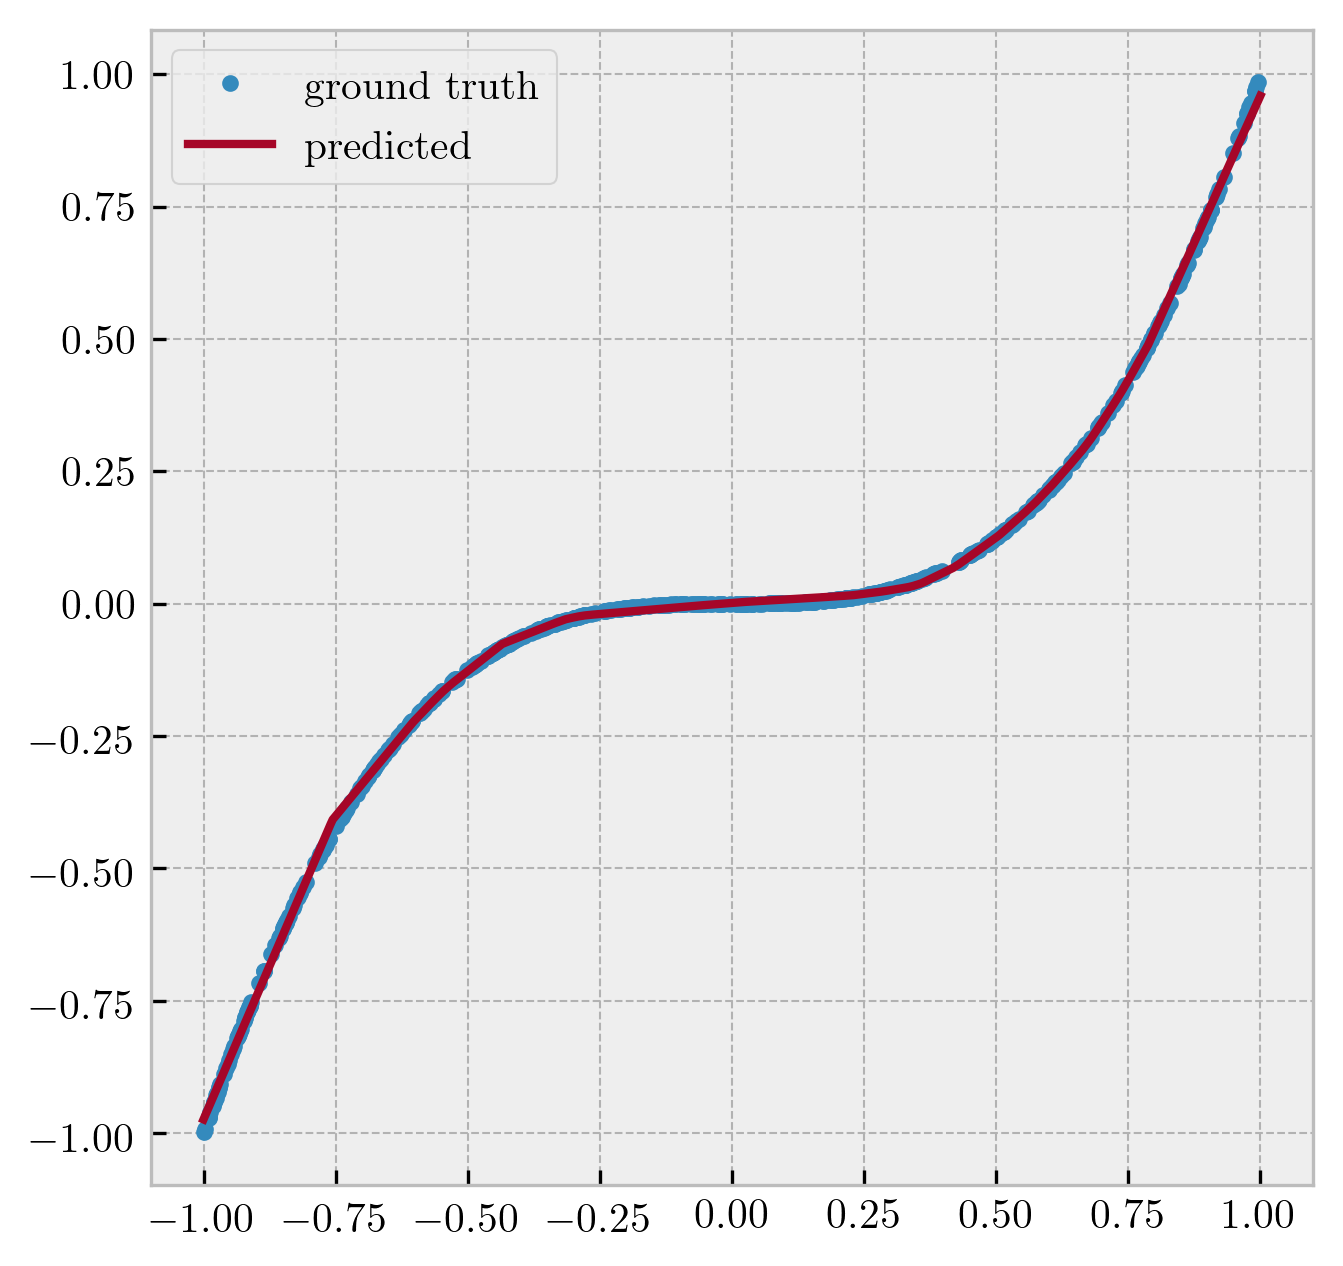
\includegraphics[width=\textwidth]{fit-3-pred.png}
		\caption{cubic}
		\label{fig:cubic}
	\end{subfigure}
	\begin{subfigure}[h!]{0.3\textwidth}
		\centering
		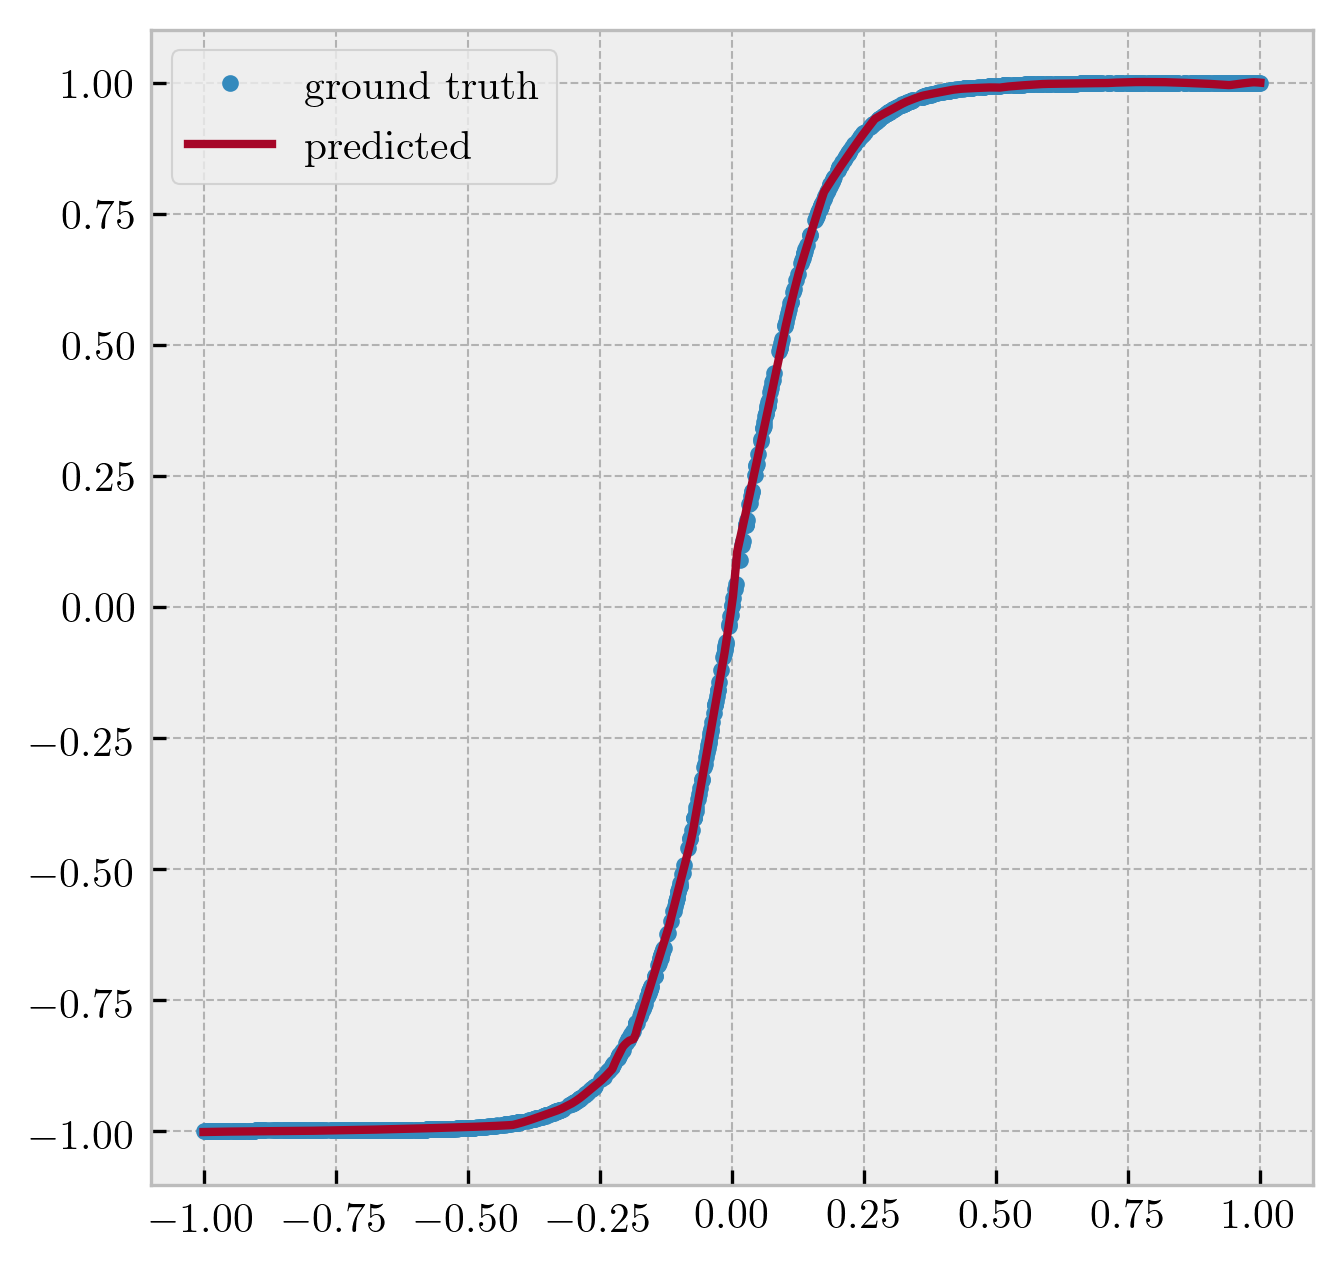
\includegraphics[width=\textwidth]{fit-tanh-pred.png}
		\caption{tanh}
		\label{fig:tanh}
	\end{subfigure}
	\begin{subfigure}[h!]{0.3\textwidth}
		\centering
		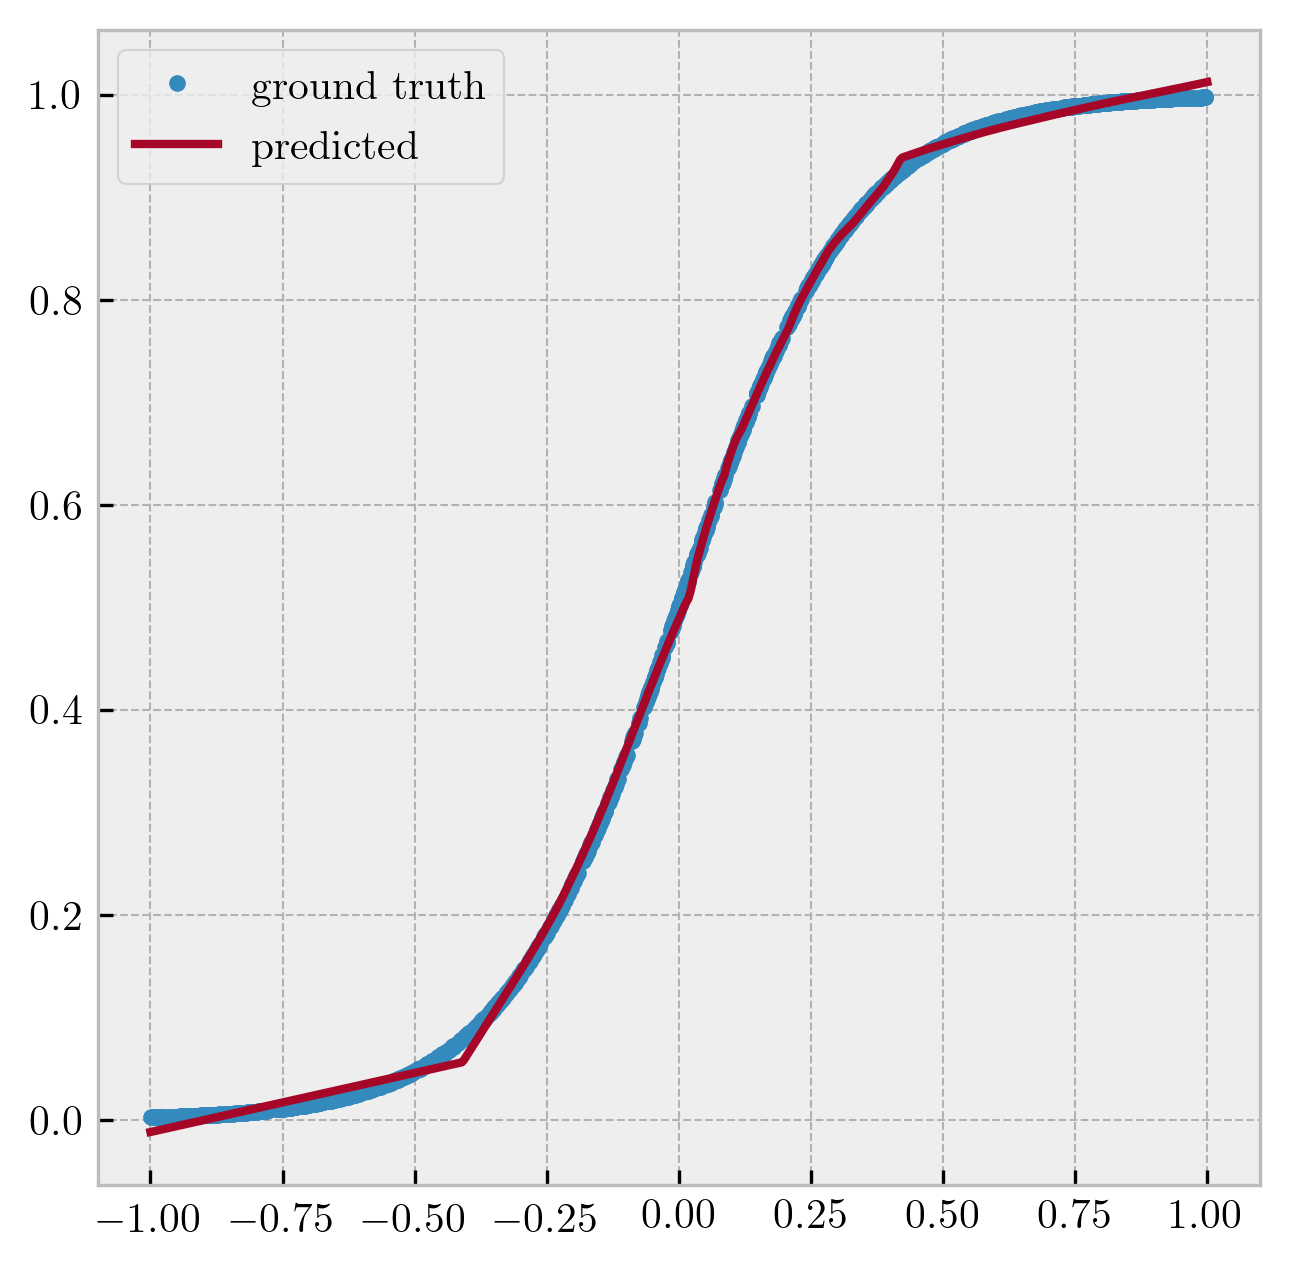
\includegraphics[width=\textwidth]{fit-sigmoid-pred.png}
		\caption{logistic sigmoid}
		\label{fig:sigmoid}
	\end{subfigure}
	\begin{subfigure}[h!]{0.3\textwidth}
		\centering
		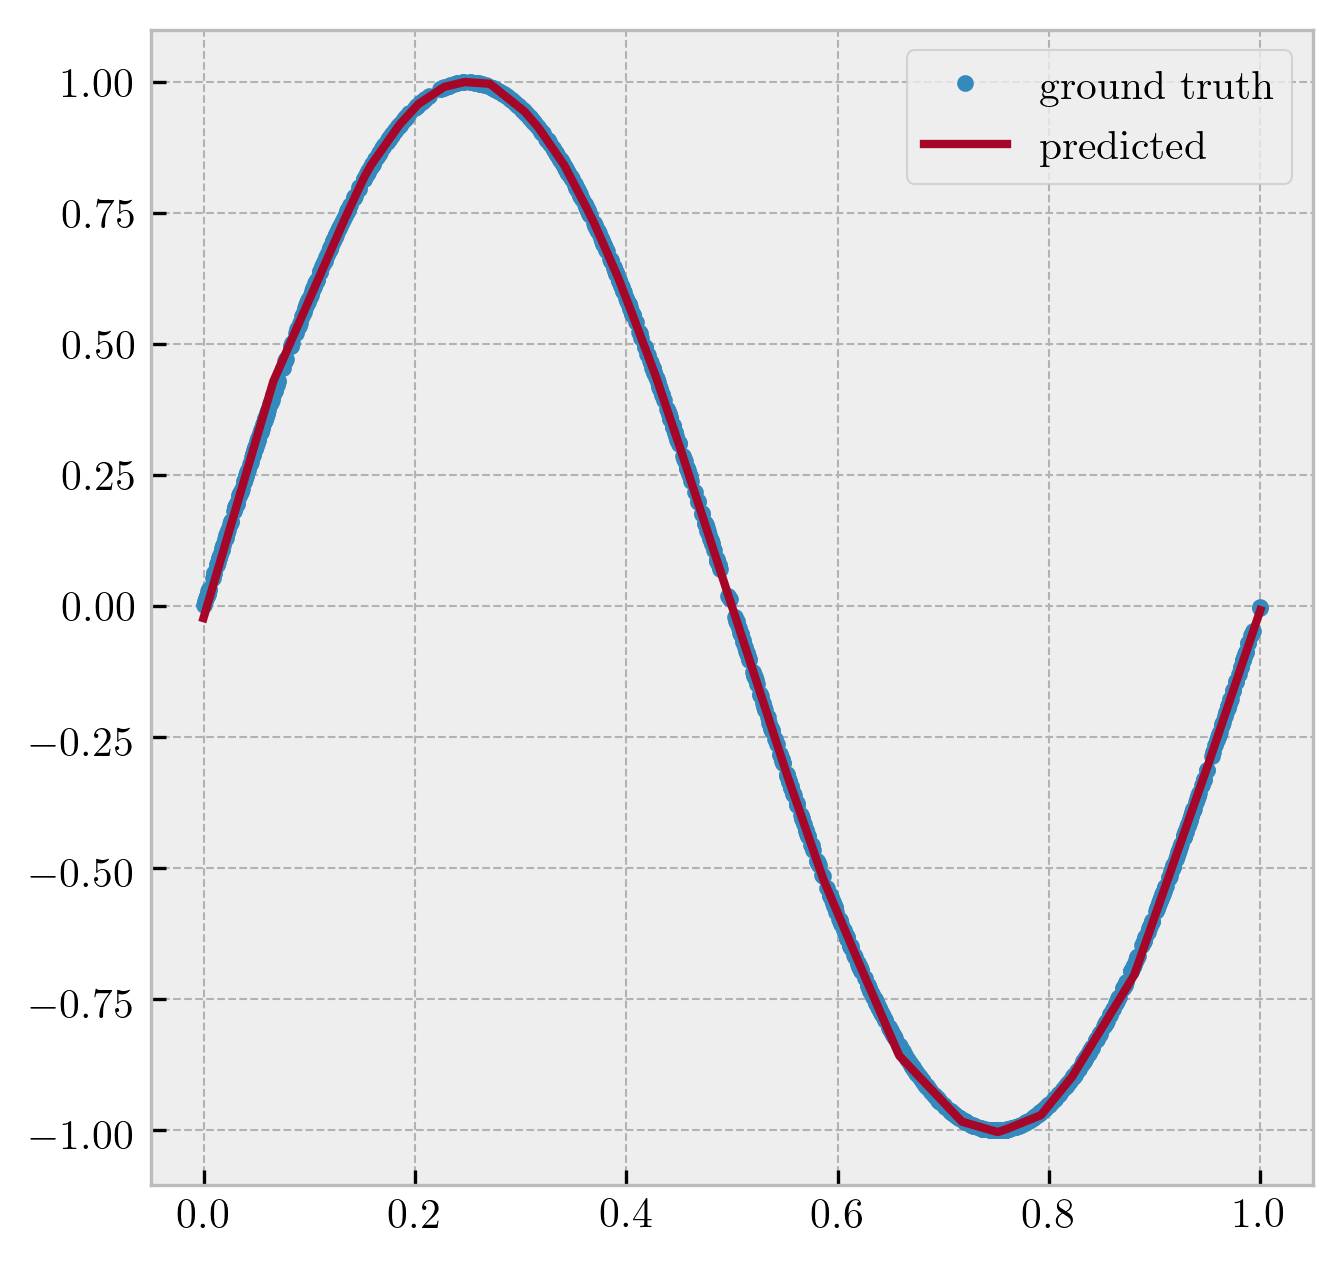
\includegraphics[width=\textwidth]{fit-sin1Hz-pred.png}
		\caption{sine}
		\label{fig:sine}
	\end{subfigure}
	\caption{Neural network as a universal function fitter.}
	\label{fig:function-fitter}
\end{figure}

The first hidden layer of the network contains 500 nodes, which are all activated by a rectified linear unit (ReLU), defined by

\begin{align}
	g(x) &= \max(0, x) \label{eq:relu} \\
	g^\prime(x) &=
	\begin{cases}
		0 & , \quad x < 0 \\
		1 & , \quad x > 0
	\end{cases} \label{eq:relu-grad}
\end{align}

\noindent The second hidden layer contains 10 nodes, also activated by ReLU. The output layer is a single node which maps everything calculated so far to a single output value. Thus, the function arguments (random numbers $\in [-1,1]$) comprise an entire dataset $\mathcal{M}$. The network objective is to minimize the $\ell_2$ loss, defined as

\begin{equation}\label{eq:l2-loss}
	\ell_2(\vec{y}, \hat{\vec{y}}) = \frac{1}{2} \norm{\hat{\vec{y}} - \vec{y}}_2^2
\end{equation}

\noindent where $\vec{y}, \hat{\vec{y}}$ are the ground truth and predicted outputs, respectively, and $\norm{\vec{y}}_2 := \qty(\sum_i y_i^2)^{1/2}$ is the $\ell_2$ norm operator. The network is trained until the loss drops below a value of 0.01. I opted to use the $\ell_2$ loss instead of the sum-of-squares error or mean-squared error because, from experience, the former is more perceptually accurate. 

For the test data, I generated 1000 equally-spaced numbers in the range $[-1,1]$. Figure \ref{fig:function-fitter} shows the predictions for each function.

\subsection{Fruit classification}
For this section, I used my extracted $a^*-b^*$ color features of bananas, apples, and oranges from previous activities. The architecture I came up with is shown in Fig. \ref{fig:fruit-architecture}. The dataset consists of 50 feature vectors for each fruit (total of 150 feature vectors), which were split 80\% for training and 20\% for testing. 

\begin{figure}[htb]
	\centering
	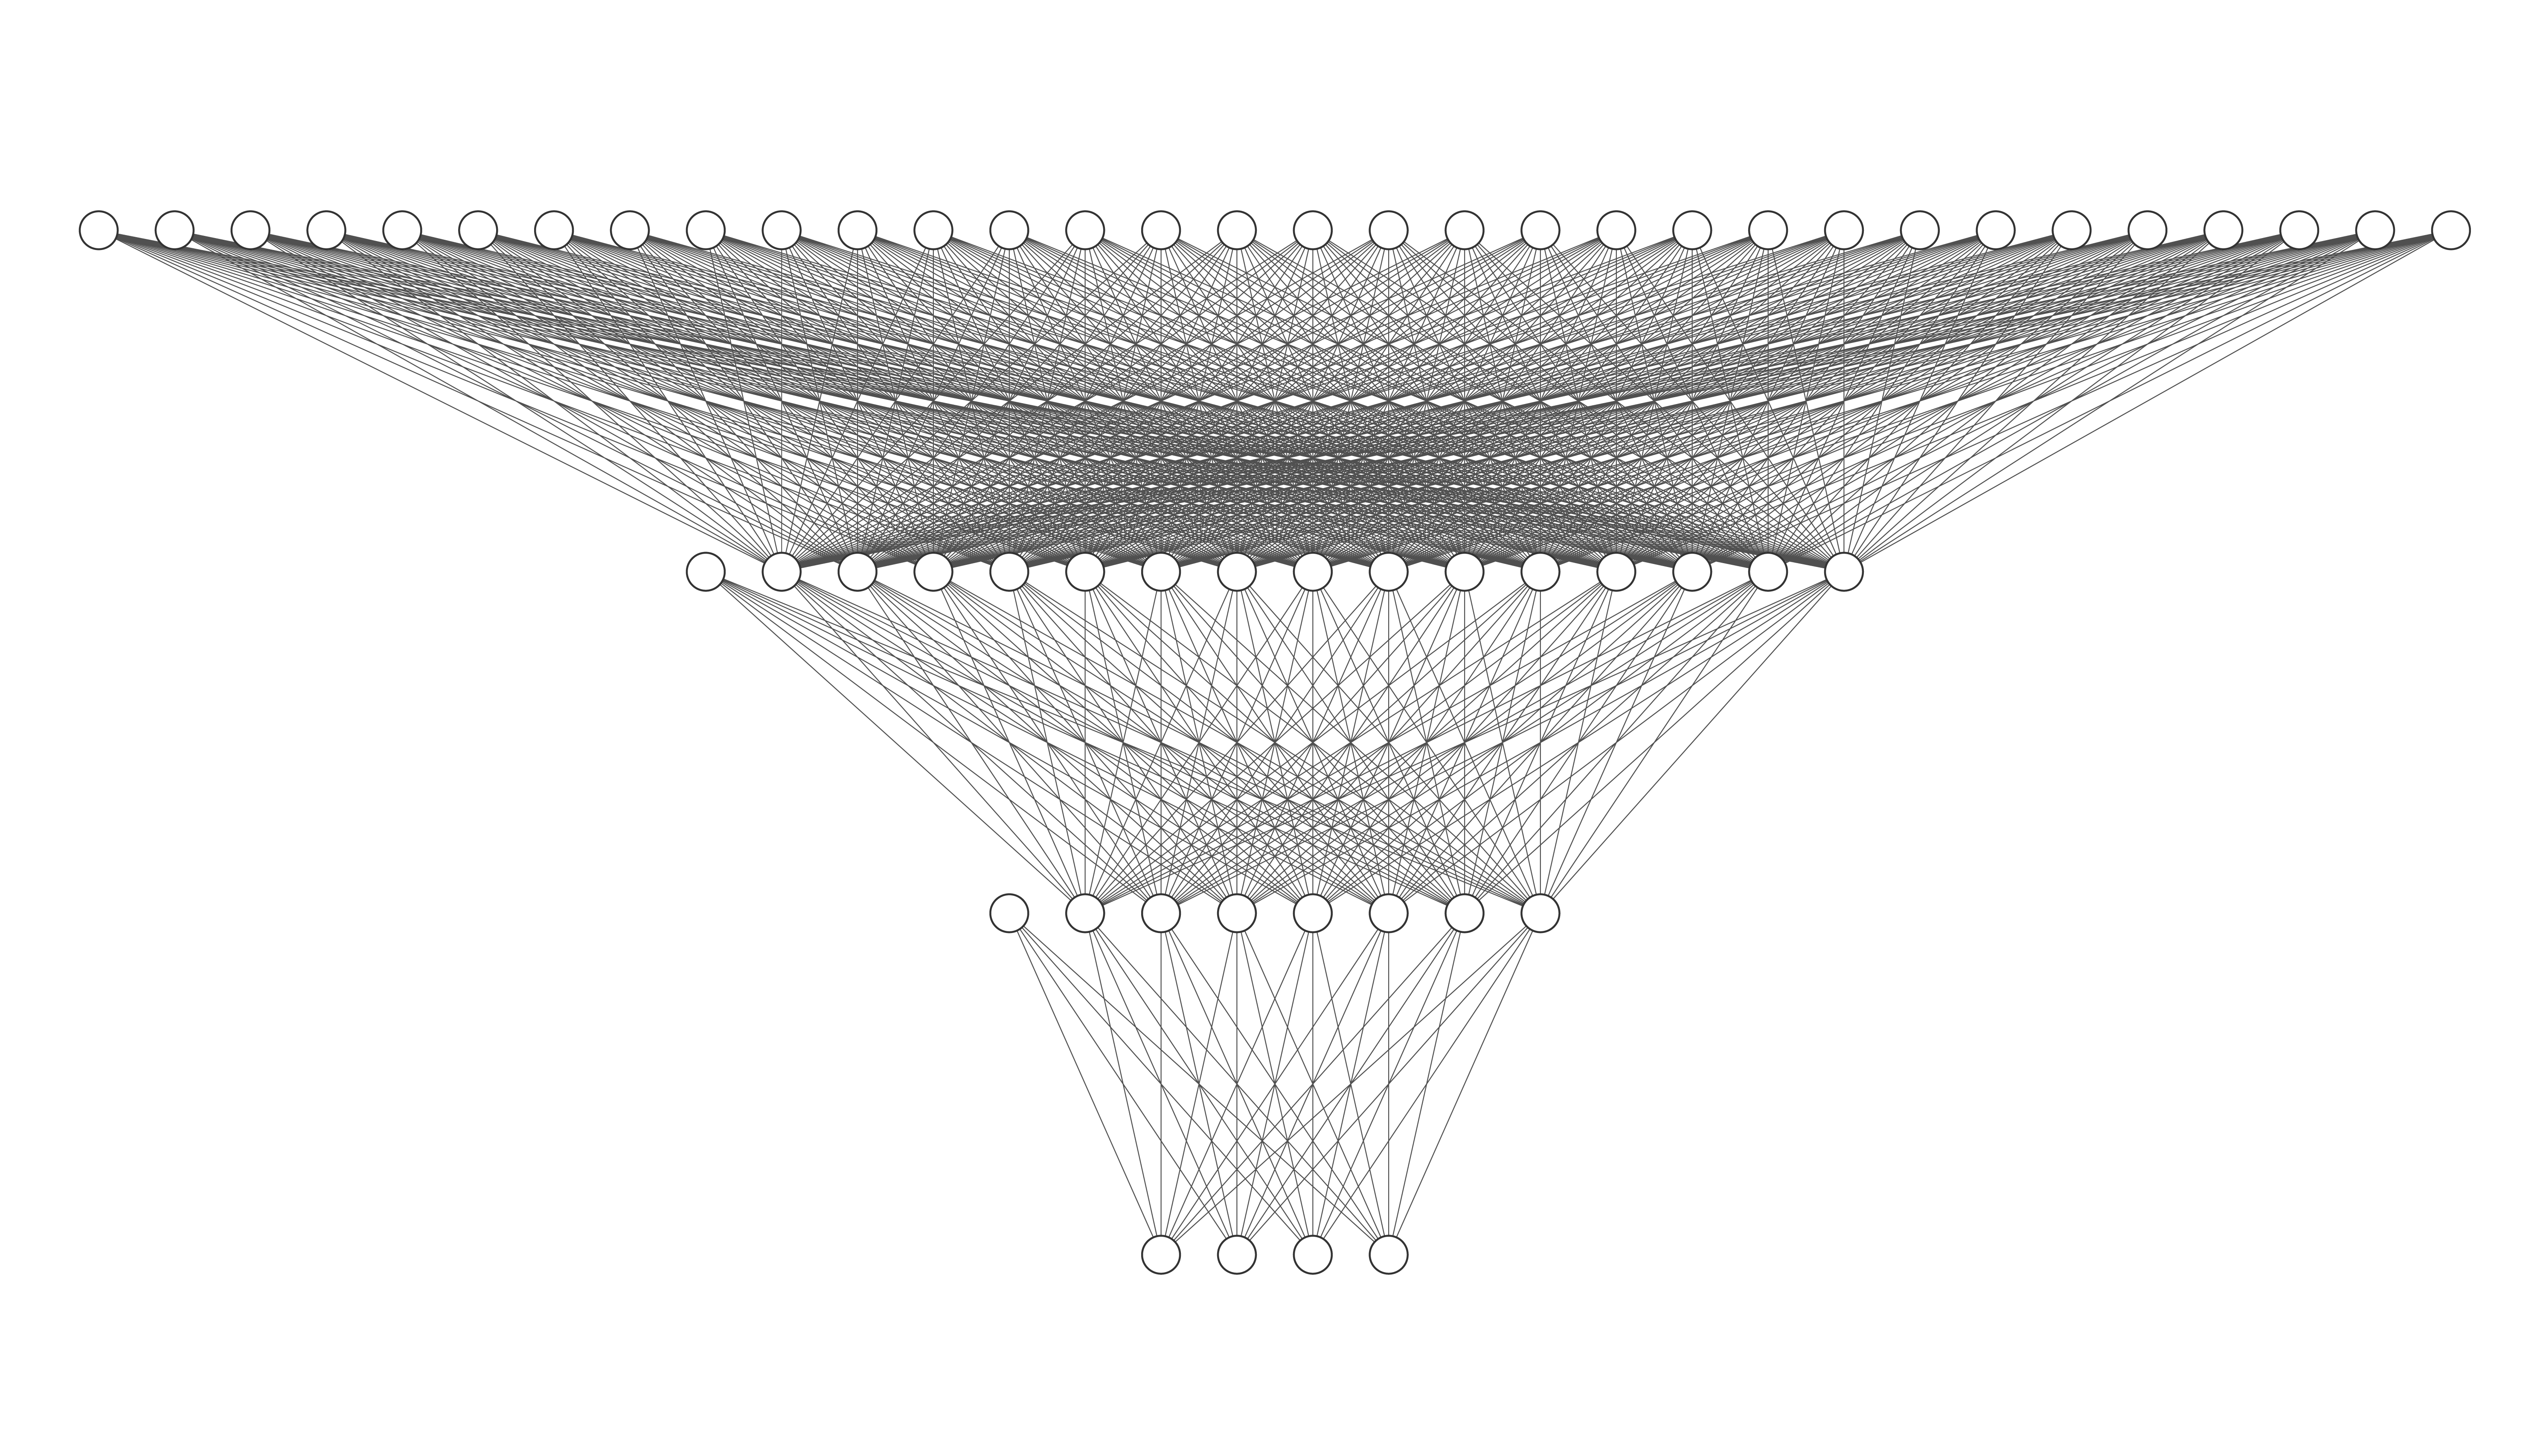
\includegraphics[width=\textwidth]{fruit-net.png}
	\caption{Network architecture for the fruit classifier.}
	\label{fig:fruit-architecture}
\end{figure}

The network was designed such that the first hidden layer contains as many nodes as data points. Layers are added which contain $\frac{1}{10}$ many nodes as the previous layer, until the number of nodes in the current layer is on the order of magnitude of $10^1$. The output layer contains as many nodes as the classes. The hidden layers are activated by a ReLU except for the last, which is activated by a logistic sigmoid, defined as

\begin{align}
	g(x) &= \frac{1}{1 + e^{-x}} \label{eq:sigmoid} \\
	g^\prime(x) &= g(x)\qty(1 - g(x))
\end{align}

\noindent and the output layer is activated by a softmax, defined by

\begin{align}
	g(x_i) &= \frac{e^{x_i}}{\sum_j e^{x_j}} \label{eq:softmax} \\
	g^\prime(x_i) &= g(x_i)\qty(\delta_{ik} - g(x_k))
\end{align}

\noindent which outputs probabilities such that the sum of the output nodes should equal unity. Thus, for this dataset, the network topology is 120-12-3 (two hidden layers, 3 nodes in output layer). 

This time, the network objective is to minimize the mean-squared error (MSE), and the network is trained until it drops below a value of 0.01. Feeding in the test data shows a test accuracy of 100\%, and the decision boundaries are shown in Fig. \ref{fig:fruit-decision3}. This is not surprising since the fruit feature vectors form distinct clusters and do not overlap.

\begin{figure}[htb]
	\centering
	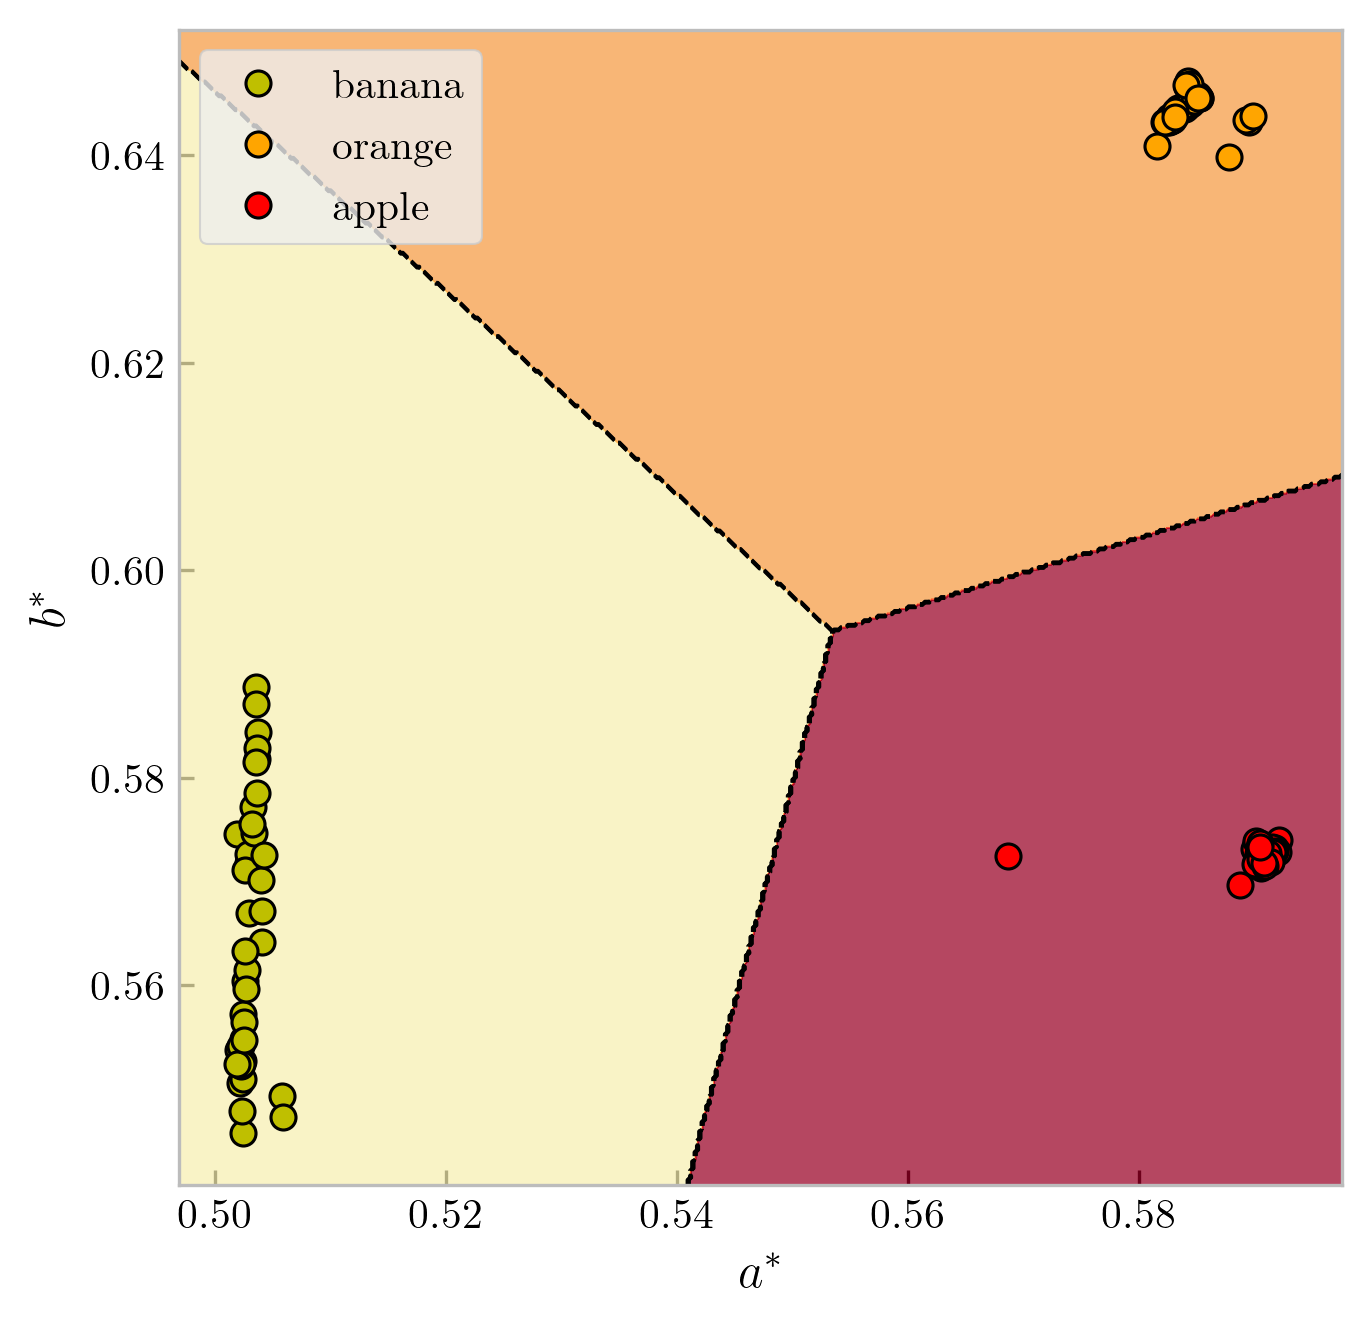
\includegraphics[width=0.7\textwidth]{ban-app-ora-decision.png}
	\caption{Decision boundaries for bananas, apples, and oranges in $a^*-b^*$ feature space.}
	\label{fig:fruit-decision3}
\end{figure}

Now, let's consider adding more samples to the training/testing sets. Using the fruits dataset from \cite{kaggle}, I added more varieties of apples, bananas, and oranges, as well as an additional class of cherries. Figure \ref{fig:fruits-set} shows the distribution of their feature vectors in $a^*-b^*$ space. Notice now that the clusters occupy more area and are almost touching each other.

\begin{figure}[htb]
	\centering
	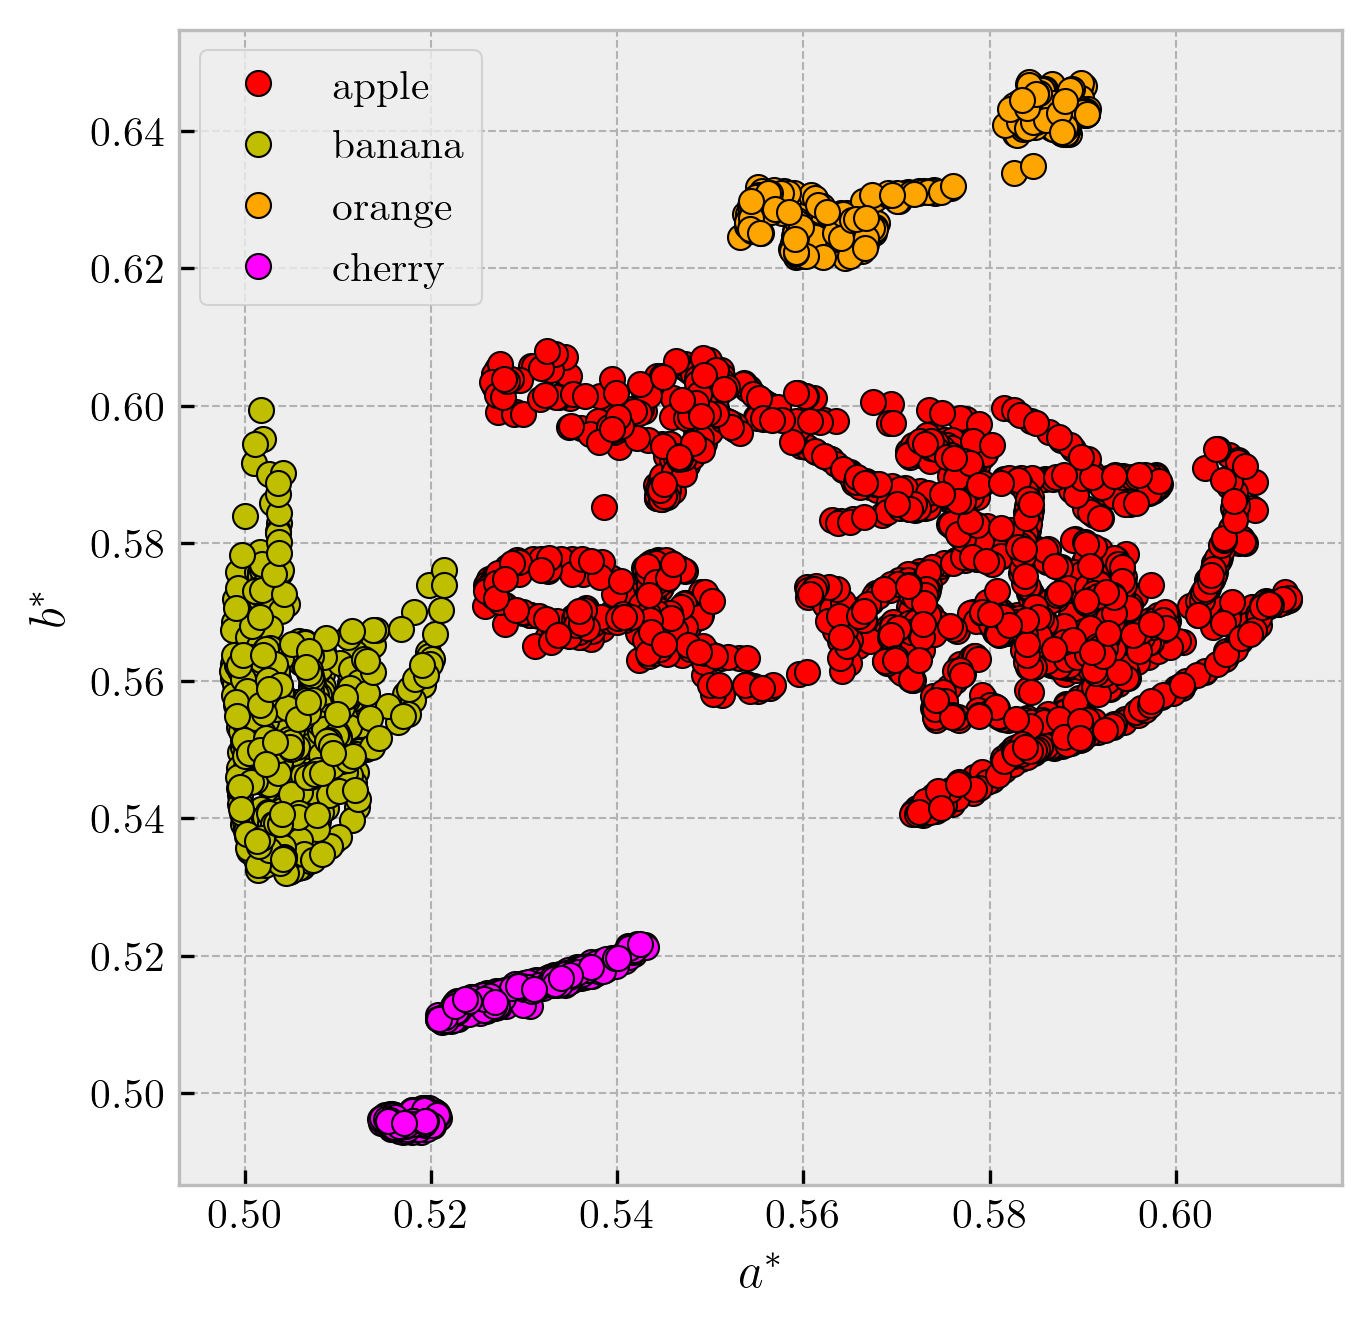
\includegraphics[width=0.7\textwidth]{fruits-train.png}
	\caption{$a^*-b^*$ feature space of apples, bananas, oranges, and cherries.}
	\label{fig:fruits-set}
\end{figure}

With a total of 4752 feature vectors, I split the data 50-50 among the train-test sets. Therefore, the network topology now is 2376-237-23-4 (3 hidden layers, 4 output nodes). Plugging in the test data afterwards yields a test accuracy of 99.96\%, and the decision boundaries are shown in Fig. \ref{fig:multiple-fruits}.

\begin{figure}[htb]
	\centering
	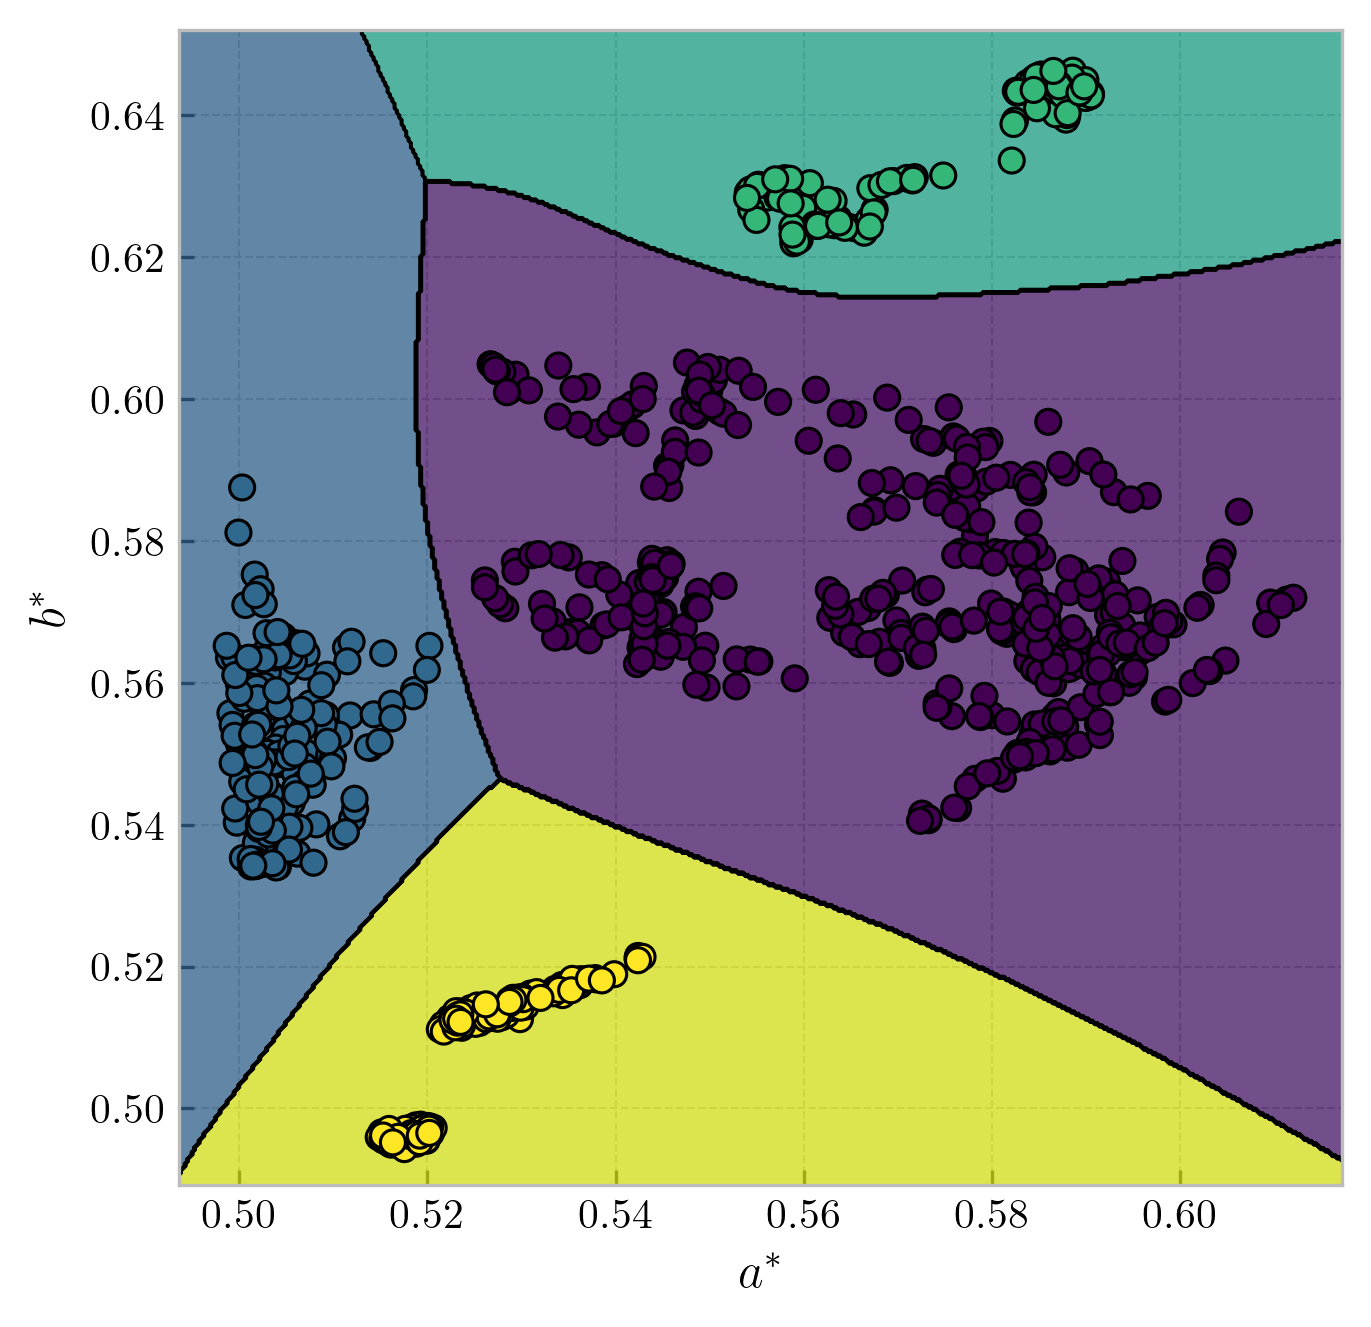
\includegraphics[width=0.7\textwidth]{multiple-decision.png}
	\caption{Decision boundaries for bananas, apples, oranges, and cherries in $a^*-b^*$ feature space.}
	\label{fig:multiple-fruits}
\end{figure}

\clearpage
\begin{table}[!htb]
	\centering
	\caption{Self-evaluation.}
	\begin{tabular}{||r|c||}
		\hline
		Technical correctness & 5 \\ \hline
		Quality of presentation & 5 \\ \hline
		Initiative & 2 \\ \hline
		\textbf{TOTAL} & \textbf{2} \\ \hline
	\end{tabular}
	\label{tab:self-eval}
\end{table}

\bibliographystyle{spp-bst}
\bibliography{biblio}

\end{document}